\documentclass[14pt]{amsart}
%\usepackage{amsmath}
\usepackage[utf8]{inputenc}
\usepackage{graphicx}
\usepackage{xcolor}
\usepackage[legalpaper, margin=1.0in]{geometry}
\usepackage{fancyvrb}
\usepackage{cprotect}
\usepackage{url}
\usepackage{etoolbox}
\usepackage{hyperref}
\usepackage[skins,theorems]{tcolorbox}
\usepackage{enumitem}
\newcommand*{\vertbar}{\rule[-1ex]{0.5pt}{2.5ex}}
\newcommand*{\horzbar}{\rule[.5ex]{2.5ex}{0.5pt}}
\setlist[itemize]{align=parleft,left=1pt..1em}

\usepackage{imakeidx}
\makeindex


\usepackage{cmbright}
\usepackage[OT1]{fontenc}


% fonts
%\input{ArtNouvc.fd}
%\newcommand*\initfamily{\usefont{U}{ArtNouvc}{xl}{n}}
%\usepackage[T1]{fontenc}
%\usepackage{tgbonum} % change font

%\usepackage[light,condensed,math]{iwona}
%\usepackage[T1]{fontenc}

% from https://www.pinterest.co.uk/pin/88664686405122253/
\definecolor{C1}{RGB}{141, 125, 158} %purple
\definecolor{C2}{RGB}{163,156,147} % yellow
\definecolor{C3}{RGB}{99,151,153} % green
\definecolor{C4}{RGB}{195,106,99} % red
\definecolor{C5}{RGB}{124, 132, 128}
\definecolor{C6}{RGB}{67, 69, 75}


\definecolor{Gr}{HTML}{377D71}
\definecolor{Pu}{HTML}{A459D1}
\definecolor{Bl}{HTML}{4D455D}
\definecolor{Te}{HTML}{C1ECE4}
\definecolor{Or}{HTML}{EF6262}
\definecolor{Am}{HTML}{F3AA60}
\definecolor{Co}{HTML}{3C486B}
\definecolor{Wh}{HTML}{FEFBF6}
\definecolor{Ye}{HTML}{FFE196}
\definecolor{Re}{HTML}{E96479}
\definecolor{Pi}{HTML}{FFD0D0}
\definecolor{Rp}{HTML}{FF9EAA}
\definecolor{Wg}{HTML}{EEF3D2}


\hypersetup{
    colorlinks=false,
    linkcolor=red,
    filecolor=red,      
    urlcolor=red,
    pdftitle={a},
    pdfpagemode=FullScreen,
    }
    
    
 % TCOLORBOX STUFF ----------------------------------------------------------------------------
 

 %  ----------------------------------------------------------------------------
    
\patchcmd{\section}{\normalfont}{\color{C5}}{}{}
\patchcmd{\subsection}{\normalfont}{\color{C5}}{}{}


\newcommand{\dfn}[1]{{\bf  \color{blue}{#1}}}


\renewcommand{\FancyVerbFormatLine}[1]{\color{gray}{>\,\,#1}}
    
\newtheorem{thm}{Theorem}


\newtheoremstyle{exercise}
{}                % Space above
{}                % Space below
{\color{black}}        % Theorem body font % (default is "\upshape")
{}                % Indent amount
{\bfseries}       % Theorem head font % (default is \mdseries)
{:}               % Punctuation after theorem head % default: no punctuation
{ }               % Space after theorem head
{}                % Theorem head spec
\theoremstyle{exercise}
\newtheorem{exercise}{Exercise}


\newtheoremstyle{example}
{}                % Space above
{}                % Space below
{\color{red}\slshape}        % Theorem body font % (default is "\upshape")
{}                % Indent amount
{\bfseries}       % Theorem head font % (default is \mdseries)
{.}               % Punctuation after theorem head % default: no punctuation
{ }               % Space after theorem head
{}                % Theorem head spec
\theoremstyle{example}
\newtheorem{example}{Example}

\newtheoremstyle{solution}
{}                % Space above
{}                % Space below
{\color{C5}}        % Theorem body font % (default is "\upshape")
{}                % Indent amount
{\bfseries }       % Theorem head font % (default is \mdseries)
{:}               % Punctuation after theorem head % default: no punctuation
{\newline}               % Space after theorem head
{}                % Theorem head spec
\theoremstyle{solution}
\newtheorem*{solution}{Solution}


\newcommand{\mcS}{\mathcal S}
\newcommand{\mcR}{\mathcal R}
\newcommand{\mcC}{\mathcal C}
\newcommand{\bS}{{\boldsymbol S}}
\newcommand{\bR}{{\boldsymbol R}}
\newcommand{\bC}{{\boldsymbol C}}
\newcommand{\ba}{{\boldsymbol a}}
\newcommand{\bb}{{\boldsymbol b}}
\newcommand{\bs}{{\boldsymbol s}}
\newcommand{\bff}{{\boldsymbol f}}
\newcommand{\br}{{\boldsymbol r}}
\newcommand{\bx}{{\boldsymbol x}}
\newcommand{\bt}{{\boldsymbol t}}
\newcommand{\bv}{{\boldsymbol v}}
\newcommand{\bu}{{\boldsymbol u}}
\newcommand{\bw}{{\boldsymbol w}}
\newcommand{\bc}{{\boldsymbol c}}
\newcommand{\be}{{\boldsymbol e}}
\newcommand{\bq}{{\boldsymbol q}}
\newcommand{\bphi}{{\boldsymbol \phi}}
\newcommand{\brho}{{\boldsymbol \rho}}
\newcommand{\btau}{{\boldsymbol \tau}}
\newcommand{\reals}{\mathbb R}
\newcommand{\ints}{\mathbb N}
\newcommand{\E}{\mathbb E}
\newcommand{\Prob}{\mathbb P}


%%%%%%%%%%%%%%%




\begin{document}



\title{Evaluating model predictions and machine learning }
\maketitle
\tableofcontents
%----------------------------------------------------------------------------------------------------------------
%\section{Reading}
%\begin{itemize}
%\item  \cite[Section 10.1]{islp}
%\begin{itemize}
%\item Example 10.1.2. This is the linear regression model with multiple predictors. 
%\item This entire section is useful and all the exercises are good practice. 
%\end{itemize}
%\item \cite[Section 10.2]{tabak}
%\item \cite[Section 10.5]{tabak}
%\item \cite[Section 3.2]{islp}
%\end{itemize}

%----------------------------------------------------------------------------------------------------------------
\section{Learning objectives}

\begin{itemize}
\item Cross validation and how to use it to perform model selection. 
\item Bias-variance decomposition of mean-squared error, and why it explains the U-shaped test error curve. 
\item Fourier series as linear regression models. Orthogonality and why it is important. 
\end{itemize}



%\begin{figure}[h!]
%    \centering
%    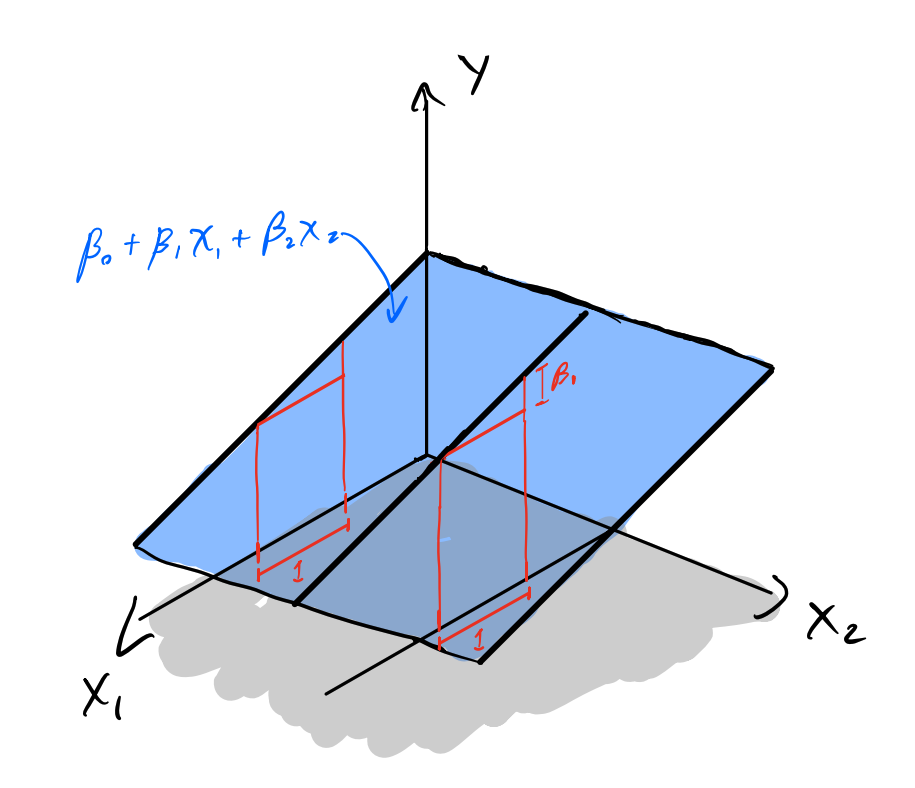
\includegraphics[width=0.8\textwidth]{./../figures/plane}
%    \caption{The function $y(x_1,x_2)$}
%    \label{fig:plane}
%\end{figure}


%----------------------------------------------------------------------------------------------------------------
\section{Cross validation}
\begin{itemize}
\item We saw from the previous example that $R^2$ is not very helpful if we want to decide how complex we'd like to make our model, since it is possible to explain all the variation in the $Y$ values with a model which is too complex. In order to address this, we take the approach of \dfn{cross validation}. The basic idea of cross validation is to break our data up into two subsets: \dfn{training set}, which we use to fit the model, and a \dfn{testing set}, which we compare to the predictions of the fitted model. 
\item {\bf Some Notation}
\begin{itemize}
\item I will use $D$ to refer to our entire data set:
\begin{equation*}
D = (Y,X) = \{(X_1,Y_1),\dots,(X_N,Y_N)\}
\end{equation*}
\item $D^{\rm train} = (Y^{\rm train},X^{\rm train})$ and $D^{\rm test} = (Y^{\rm test},X^{\rm test})$ will represent the subsets of the data to be used to training (that is, fitting) the model and testing the fit respectively.  We will assume that
\begin{equation*}
D = D^{\rm train} \cup D^{\rm test}
\end{equation*}
 Let $N_{\rm train}$ and $N_{\rm test}$ denote the number of points in each group.
 \item Let $\hat{y}(x,D)$ the prediction of $E[Y|X =x]$ using the fitted coefficients based on a data set $D$; that is
\begin{equation*}
\hat{y}(x,D) = \sum_{i=1}^{K}\hat{\beta}_i\phi_i(x)
\end{equation*} 
where $\hat{\beta}$ are the (usually least squares) fitted coefficients using the data in $D$. 
\end{itemize}




\item  
Now let us define the \dfn{training error}
\begin{equation*}
\epsilon_{\rm train}^2=  \frac{1}{N_{\rm train}}\sum_{i=1}^{N_{\rm train}}(\hat{y}(X_i^{\rm train},D^{\rm train}) - Y_i^{\rm train})^2
\end{equation*}
where the average is taken over different replicates of our data and $\hat{Y}_i$ is our prediction of $E[Y|X]$. Not that the training error tells us about how well our model does at predicting the same data we used to fit it, and therefore not surpisingly, it is closely related to $R^2$:
\begin{equation*}
R^2 \approx 1 - \frac{\epsilon_{\rm train}^2}{{\rm var}(Y_{{\rm train},i})}.
\end{equation*}

In order to see how well our model does at predicting the points we did NOT use to fit it, we introduce the test error: 
\begin{equation*}
\epsilon_{\rm test}^2=  \frac{1}{N_{\rm test}}\sum_{i=1}^{N_{\rm test}}(\hat{y}(X_i^{\rm test},D^{\rm train}) - Y_i^{\rm test})^2
\end{equation*}
Note that the fitted coefficients used to compute $\hat{y}_i(X^{\rm test})$ come from fitting the model to the training data, even though we are evaluating $\hat{y}$ at the test points. 

\begin{example}[Cross validation on polynomial model]\label{ex:polycrossval}
Consider example 6 from the previous weeks notes. \\

\noindent
\underline{Question:} Plot the training and test error as a function of the number of parameters. \\

\noindent
\underline{Solution:}  See \href{https://colab.research.google.com/drive/1EYcMviowfsnsVe7vsUKlyzkNsddUiTau?usp=sharing}{colab notebook}.
\end{example}
\end{itemize}

%----------------------------------------------------------------------------------------------------------------
\section{Bias, variance and overfitting}
\begin{itemize}


\item In order to understand U-shaped curve seen in Example \ref{ex:polycrossval},  we first need to introduce some more general terminology and notation for talking about estimators (of which $\hat{y}$ is an example). 
To this end, we introduce the \dfn{mean-squared error} of an estimator $\hat{\theta}$ of some quantity $\theta$. $\theta$ could be a parameter, or it could be a value of a function, such as $f(x)$, that we would like to predict. 
\begin{equation}\label{eq:mse}
{\rm MSE}_{\hat{\theta}}= E\left[(\hat{\theta}- \theta)^2\right]
\end{equation}
 For now, let's just think of $\hat{\theta}$ as any estimator. 
\item The following theorem is the key result which will allow us to understand the U-shaped curve. 
\begin{thm}[Bias variance decomposition]
\begin{equation}\label{eq:biasvar}
{\rm MSE}_{\hat{\theta}} = {\rm var}(\hat{\theta}) + E\left[\hat{\theta}-\theta\right]^2
\end{equation}
\end{thm}
\begin{proof}
Using the definition of variance 
\begin{equation*}
{\rm var}\left(\hat{\theta}-\theta\right) = E\left[(\hat{\theta}-\theta)^2\right] - E\left[\hat{\theta}-\theta\right]^2. 
\end{equation*}
Since $\theta$ is a constant, ${\rm var}\left(\hat{\theta}-\theta\right)= {\rm var}\left(\hat{\theta}\right)$, so 
rearranging terms yields the result. 
\end{proof}
Now let's break this result down a bit. 
\begin{itemize}


\item  The first term in Equation \ref{eq:biasvar} is simply the variance, which in the case of an estimator of a parameter we can recognize as the squared standard error. This is tell us how much variation there is in our estimate from replicate of replicate. You should recognize that a consistent estimator is exactly one for which this quantity vanishes when $N$ is very large. 
\item The second term is what we will define as the squared of the bias: 
\begin{equation*}
{\rm Bias}_{\hat{\theta}} = E[\hat{\theta}-\theta].
\end{equation*}
This tell us whether our estimate will on average give us the correct value of $\theta$. You should recognize that an unbiased estimator is exactly one for which this quantity is zero!
\end{itemize}
\item Now let's return to working in the context of a model of the form 
\begin{equation*}
Y|X \sim {\rm Normal}(f(X),\sigma^2)
\end{equation*}
where $f(X)$ can be written as a linear combination of features
\begin{equation*}
f(X) = \sum_{i=1}^N\beta_i \phi_i(X). 
\end{equation*}
Letting $\hat{\theta} = \hat{y}(x,D)$, applying Equation \ref{eq:mse} yields
\begin{equation*}
{\rm MSE}_{\hat{y}(x,D)} = E\left[(\hat{y}(x,D)- f(x))^2\right]
\end{equation*}
where the average is taken over replicates of our data $D$. This is a measurement of our ability to predict $f(x)$, which is exactly what the test error seeks to measure. 
\item  To more closely relate the bias-variance tradeoff to the test error, we will use a slightly different definition of MSE, which is 
\begin{equation}\label{eq:tilMSE}
\widetilde{{\rm MSE}}_{\hat{y}(x,D)} = E\left[(\hat{y}(x,D)- Y(x))^2\right]
\end{equation}
where $Y$ is a sample from $Y|(X=x)$. You can show (see Exercise) that
\begin{equation*}
\widetilde{{\rm MSE}}_{\hat{y}(x,D)} = \sigma^2 +{\rm var}(\hat{y}(x,D)) + E\left[\hat{y}(x,D)-f(x)\right]^2
\end{equation*}
The new term, $\sigma^2$, captures the fact that, unlike the deterministic term $f$, we can NEVER predict the \emph{random} variable $Y$ exactly. 
You should be able to justify that
\begin{equation*}
\epsilon_{\rm test}^2 \approx E\left[\widetilde{{\rm MSE}}_{\hat{y}(X,D^{\rm train})}\right]
\end{equation*}
\item The important thing to recognize is that a complicated model will tend to have a higher variance, since it will be able to change more in response to data. Meanwhile, a very simple model will tend to have a higher bias. 



\begin{example}[Plotting Bias and variance]

Let's continue with Example \ref{ex:polycrossval} and try to illustrate the bias variance tradeoff by computing these (or really approximations to them) separately. \\


\noindent
\underline{Solution:}  See \href{https://colab.research.google.com/drive/1EYcMviowfsnsVe7vsUKlyzkNsddUiTau?usp=sharing}{colab notebook}.

\end{example}

\item We now summarize some observations we've made thus far:
\begin{itemize}
\item In a regression model, as we add more coefficients, eventually the model becomes more and more ``flexible'', in the sense that is can describe more different types of data sets. Here, by ``describe'', we mean that it can be fit to those data sets with a small value of $R^2$ or training error.  With enough features, a model can perfectly interpolate between the data points, meaning $\hat{y}(X_i,D) = Y_i$ for each data point $(X_i,Y_i)$ when the model is fit on all our data points. 
\item Unlike the training error and $R^2$, the test error, $\epsilon_{\rm test}^2$ does not simply increase as we make the model more complex, rather it has a U-shape. Thus, there is a optimal model size at which our model's predictions of new data points -- that is, data points outside the set we used to fit it -- is best. 
\item The $U$-shape can be understood in terms of bias and variance. We know this because the mean-squared error, which is the ``math world'' version of $\epsilon_{\rm test}^2$, can be decomposed into a bias and variance term. The variance term tells us how variable the predictions of our model will be when we fit it to different training sets, while the bias tells us how much its predictions. will differ, on average, from real data. 
\end{itemize}

\begin{figure}[h]
    \centering
    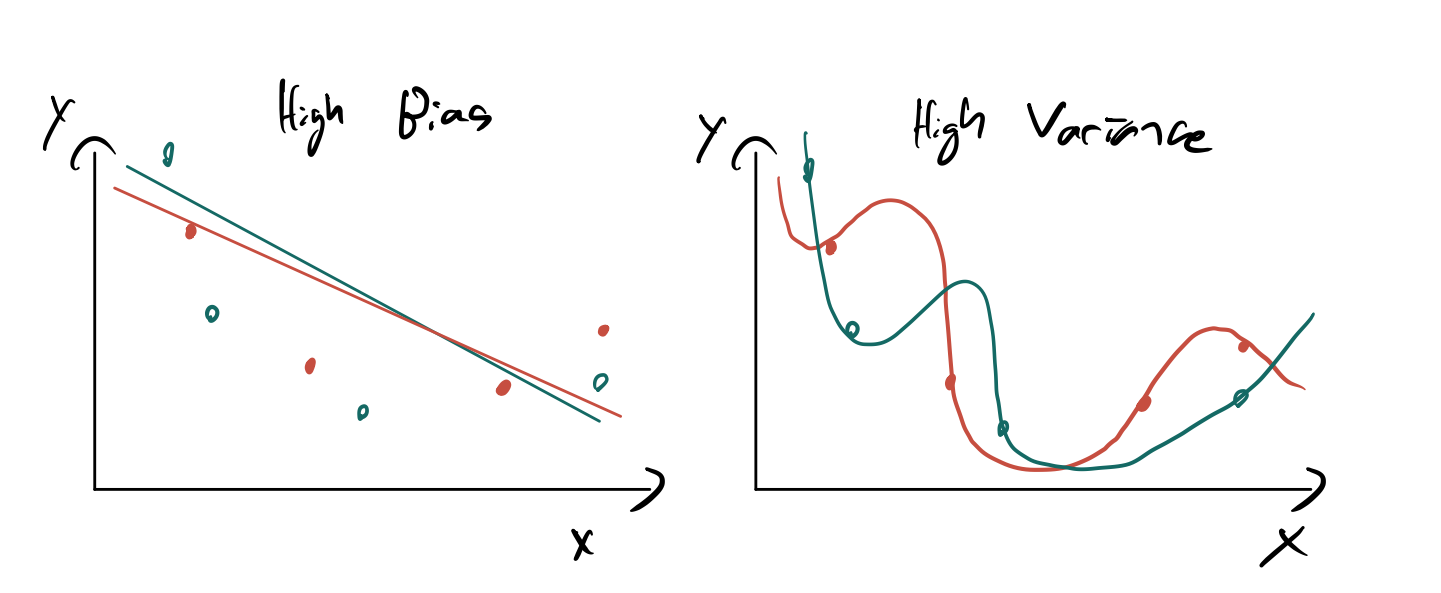
\includegraphics[width=0.8\textwidth]{./../figures/bias_var}
    \caption{Bias and variance illustrated with fits to two different datasets (blue and red) drawn the from the same distribution}
    \label{fig:bv}
\end{figure}



\end{itemize}



\section{Orthogonality and Fourier analysis}
\begin{itemize}
\item Sometimes we have a particularly hypothesis about what features my contribute to an signal we are analyzing -- for example, the CO2 data from last week we suspected there was a linear trend and yearly trend superimpose together. This was reasonable because we know that whether tends to follow a yearly cycle. But in general, if we don't have such knowledge how should we select the functions $\phi$?  It is often to our advantage to select basis function $\phi_i$ so that our predictors are not correlated. That is, if $\phi_i(X)$ and $\phi_j(X)$ are thought of as random variables (the randomness comes from $X$) then we want them to be uncorrelated. 



\item Throughout our discussion, we will assume that $E[\phi_i(X)]=0$. We can easily make this so by subtracting the means of our features. Therefore, we would like to find $\phi_i$ such that 
\begin{equation}\label{eq:orth}
E[\phi_i(X)\phi_j(X)] = 0 \quad i\ne j.
\end{equation}
We this holds for some distribution of $X$, we say that $\phi_i$ and $\phi_j$ are \dfn{orthogonal} with respect to this distribution.



\begin{example}[Sin series]\label{ex:sin}

Let us now work with the particular example where 
\begin{equation}\label{eq:Xunif}
X \sim {\rm Uniform}(-L,L).
\end{equation}
Even if our $X$ points are not random, but are say evenly spaced on the interval $[-L,L]$, a random sample from the uniform distribution will be statistical similar to some randomly selected evenly spaced $X$ points. Thus, we can think of the uniform distribution as approximating the spread of our $X$ data with a random variable. 

Now consider the basis functions 
\begin{equation*}
\phi_j(x) = \sin\left(\frac{\pi x j}{L} \right).
\end{equation*}

 


\noindent
\underline{Question:} Show using simulations that $\phi_j$ are orthogonal with respect to the uniform distribution on $[-L,L]$ (Equation \ref{eq:Xunif}). \\


\noindent
\underline{Solution:}  See \href{https://colab.research.google.com/drive/1EYcMviowfsnsVe7vsUKlyzkNsddUiTau?usp=sharing}{colab notebook}.

\end{example}



\item Notice that if $\phi_j$ are orthogonal, then we can express the regression coefficients as
\begin{equation*}
\beta_j = \frac{{\rm cov}(Y,\phi_j(X))}{{\rm var}(\phi_j(X))} =  \frac{E[Y\phi_j(X)]}{E[\phi_j(X)^2]}
\end{equation*}
and hence our fitted coefficients from $N$ data points can be approximated as
\begin{equation}\label{eq:fourier_coef}
\hat{\beta}_j \approx \frac{\sum_{i=1}^N\phi_j(X_i)Y_i}{\sum_{i=1}^N\phi_j(X_i)^2}
\end{equation}
This suggests $\hat{\beta}_j$ should depend only weakly how many of the features $\phi$ we have included in our model! This is consequence of orthogonality. In contrast,  in the earlier example where we used polynomial features adding a new predictor, say $X^4$, would dramatically change the fitted value of $\beta_2$. However, 
\item Now let's return to Example \ref{ex:sin}. A limitation of this model is that it only permits us to model ``odd functions'' that is, functions for which $f(x) = -f(x)$, as each $\phi_j$ has this property. It is therefore desirable to add addition features which permit this, but we'd like them to still be orthogonal. To this end, we introduce a new set of features to the model given by the cosine functions:
\begin{equation*}
 \cos\left(\frac{\pi x j}{L} \right).
\end{equation*} 
Our new model, called a \dfn{Fourier series}, is given by 
\begin{equation*}
f(x) = \beta_0 + \sum_{i=1}^K\beta_i\sin\left(\frac{\pi i x }{L} \right) + \alpha_i \cos\left(\frac{\pi i x }{L} \right)
\end{equation*}
where we are using $\alpha_i$ to represent the coefficients of the cosine terms. Fourier series are on of the most important models in data science and engineering. It can be proved that as $K \to \infty$ we can approximate essentially ANY function with a series of this form.


\begin{example}[Working with Fourier series in python]\label{ex:fourier}
Suppose we have data from the model with 
\begin{equation*}
f(x) = \sin(3\pi x) + \sin (10\pi x)
\end{equation*}
where $X_i = (i-1)/N$ (meaning the $X$ points are evenly spaced in $[0,1]$. \\



\noindent
\underline{Question:} For different values of $\sigma^2$, generate data from this model and fit it to a Fourier series with $K=100$ terms. \\



\noindent
\underline{Solution:} See \href{https://colab.research.google.com/drive/1EYcMviowfsnsVe7vsUKlyzkNsddUiTau?usp=sharing}{colab notebook}. \\


\end{example} 

\item The process of computing the coefficients $\hat{\beta}_j$ and $\hat{\alpha}_j$ for the Fourier series is called  a \dfn{Discrete Fourier Transform}. Usually DFT refers to the cases where the $X_i$ are equally spaced. In this case, the orthogonality condition (Equation \ref{eq:orth}) is true is ``data world'', not just ``math word'' -- what I mean by this is that for equally spaced data points. 

To be precise, consider the predictor data on the interval $[0,L]$ given by 
\begin{equation*}
X_i = \frac{L(i-1)}{N-1}
\end{equation*}
for $i=1,\dots,N$. Thus $X_1 = 0$, $X_2 = L/N$, $X_3 = 2L/N$ and $X_N = L$. We could generate these points with \verb!np.linspace!. The following theorem tells us that the empirical, or sample covariance between the sin features, is exactly zero for these predictors.

\begin{thm}
\begin{equation*}
\sum_{i=1}^N\sin\left(\frac{2\pi j X_i}{L}\right) \sin\left(\frac{2\pi k X_i}{L}\right)  =0\quad k\ne j
\end{equation*}
\end{thm}

%\begin{proof}
%To prove this you would use the identity 
%\begin{equation*}
%\sin(x)\sin(y) = \frac{1}{2}(\cos(x-y) - \cos(x+y))
%\end{equation*}
%\end{proof}

\item Often we want to summarize how different frequencies are represented in our data, but we don't particularly care about whether they come form the $\sin$ or $\cos$ terms. To achieve this, one uses the \dfn{power spectrum density}, also known as the \dfn{peridogram}, 
\begin{equation*}
P_j = \beta_j^2 + \alpha_j^2. 
\end{equation*}
The power spectrum density is a fundamental object in signal processing, and it essentially tells us how ``wobbly'' a signal is. 
%As the following example will illustrate the noisy data we have been working with extremely wobbly. 





\begin{example}[Periodogram]\label{ex:period}
\noindent
\underline{Question:} Compute the periodogram of the data generated in Example \ref{fourier} and confirm the same periodogram can be generated with the \verb!periodogram!  function from the \verb!scipy.signal! library. This is neat and not often made point, that this fundamental structure from signal processing is in fact coming from fitting a linear regression model with least square!! \\

\noindent
\underline{Solution:} See \href{https://colab.research.google.com/drive/1EYcMviowfsnsVe7vsUKlyzkNsddUiTau?usp=sharing}{colab notebook}. \\

\end{example}




\end{itemize}


 \bibliographystyle{unsrt}
\bibliography{./../refs.bib}




\end{document}



 \bibliographystyle{unsrt}
\bibliography{./../refs.bib}




\end{document}





